% Chapter Template

\chapter{M\'etodos} % Main chapter title

En este capitulo describiremos el algoritmo utilizado para la realizacion del presente trabajo final.\\

En la secci\'on 3.1 realizaremos una descripci\'on general, la misma contiene informaci\'on acerca de  los m\'etodos de segmentaci\'on propuestos para las im\'agenes de fondo de ojo utilizadas en este proyecto, el concepto de preprocesamiento de im\'agenes, la extracci\'on de indicadores y finalmente el entrenamiento y clasificaci\'on de las im\'agenes basado en indicadores.\\

En la secci\'n 3.2 nos enfocaremos en el preprocesamiento de las im\'agenes. Se detallan las caracteristicas iniciales de las im\'agenes propuestas, las t\'ecnicas utilizadas para la extracci\'on de ruido y fondo, as\'i como tambi\'en la tecnica utilizada para mejorar el contraste. Finalmente se explican los pipelines propuestos y analizados para el preprocesamiento correspondiente de las im\'agenes de fondo de ojo.\\

En la secci\'on 3.3...\\

En la secci\'on 3.4...\\
\label{Chapter3} % Change X to a consecutive number; for referencing this chapter elsewhere, use \ref{ChapterX}

%----------------------------------------------------------------------------------------
%	SECTION 1
%----------------------------------------------------------------------------------------

\section{Descripci\'on general}

Una categorizaci\'on com\'un de los algoritmos para segmentaci\'on de estructuras vasculares en im\'agenes m\'edicas incluyen t\'ecnicas, tales como enforques basados en regiones y basados en bordes, t\'ecnicas de reconocimiento de patrones, enfoques basados en modelos, enfoques basados en el seguimiento y enfoques basados en redes neuronales. Los algoritmos para la segmentaci\'on de vasos sanguineos se pueden dividir en 6 categorias principales:
\begin{itemize}
	\item T\'ecnica de reconocimiento de patrones.
	\item Filtrado adaptado.
	\item Seguimiento de vasos.
	\item Morfolog\'ia matem\'atica.
	\item Enfoques multiescala.
	\item Enfoques basados en modelos.
	\item Aproximaciones paralelas basadas en hardware.
\end{itemize}
	
La t\'ecnica de reconocimiento de patrones se divide en dos subcategorias, enfoques supervisados y enfoques no supervisado.

El m\'etodo de segmentaci\'on propuesto en el presente trabajo final es un m\'etodo supervisado. En este m\'etodo, la regla para la extracci\'on de los vasos sanguineos es aprendido sobre la base de un conjunto de formaci\'on de im\'agenes de referencia procesados y segmentados manualmente por un oftalm\'ologo. En un procedimiento supervisado, los criterios de clasificaci\'on son determinados sobre la base de caracter\'isticas dadas. Por lo tanto, el requisito previo es la disponibilidad de los datos reales ya clasificados. Como m\'etodos supervisados est\'an dise\~nados en base a los datos pre-clasificados, su rendimiento suele ser mejor que el de los m\'etodos no supervisados y puede producir muy buenos resultados para las im\'agenes retinianas saludables. \cite{fraz2012blood} \cite{akita1982computer} \cite{hoover2000locating} \\

FIGURA\\

El procesamiento digital de im\'agenes es el conjunto de t\'ecnicas que se aplican a las im\'agenes digitales con el objetivo de mejorar la calidad o facilitar la b\'usqueda de informaci\'on.\\

Durante el preprocesamiento de im\'agenes se aplican un conjunto de filtros, cuyo objetivo fundamental es obtener, a partir de una imagen inicial, otra final cuyo resultado sea mas adecuado para una aplicaci\'on espec\'ifica.

En este trabajo, el preprocesamiento tiene por objetivo:
\begin{itemize}
 \item Suavizar la imagen: reducir la cantidad de variaciones de intensidad entre p\'ixeles vecinos.
 \item Eliminar ruido: eliminar aquellos p\'ixeles cuyo nivel de intensidad es muy diferente al de sus vecinos y cuyo origen puede estar tanto en el proceso de adquisici\'on de la imagen como en el de transmisi\'on.
 \item Realzar el contraste entre los vasos sanguineos y las demas estructuras anat\'omicas que componen la retina.
\end{itemize}








%-----------------------------------
%	SECTION 2
%-----------------------------------
\section{Preprocesamiento}

La fotografía retinal requiere el uso de un complejo sistema óptico, llamado camara de fondo. Este es  un microscopio especializado  de baja potencia con una cámara adjunta, capaz de iluminar y formar imágenes de la retina simultáneamente. Está diseñado para tomar una imagen de la superficie interior del ojo, que incluye la retina, el disco óptico, mácula y polo posterior. La cámara de fondo normalmente opera en tres modos. En la fotografía a color de la retina se examina todo bajo la iluminación de luz blanca. En la fotografía libre de rojo, los vasos y otras estructuras se mejoran en contraste y la luz de la imagen se filtra para eliminar los colores rojos. Las angiografías con fluoresceína se adquieren mediante el método del colorante de rastreo. La fluoresceína de sodio y verde de indocianina se inyecta en la sangre, y luego el angiograma se obtiene fotografiando la fluorescencia emitida después de la iluminación de la retina con luz azul a una longitud de onda de 490 nanómetros.\\

La vascularización retiniana se compone de arterias y venas que aparecen como rasgos alargados, con sus afluentes visibles dentro de la imagen retiniana. Hay una amplia gama de anchos de los vasos que van desde un píxel a veinte píxeles, dependiendo de la anchura de la embarcación y la resolución de la imagen. Otras estructuras que aparecen en las imágenes de fondo de ojo incluyen el límite retina, el disco óptico, y las patologías en forma de manchas algodonosas, lesiones brillantes y oscuras y exudados como se muestra en (\ref{fig:Fondo_de_ojo} (b-d)).\\

El recipiente de perfiles de intensidad de la sección transversal se aproximan a una forma gaussiana o una mezcla de gaussianas en el caso en que un reflejo central de vasos se encuentre presente. La orientación y la escala de grises de un vaso no cambia bruscamente; que son localmente lineales y cambian gradualmente en intensidad a lo largo de su longitud. Los vasos se pueden esperar para ser conectado y, en la retina, forman un árbol binario como la estructura. Sin embargo, la forma, tamaño y nivel de gris local de los vasos sanguíneos pueden variar enormemente y algunas de las características de fondo pueden tener atributos similares a los vasos como se ilustra en (\ref{fig:Fondo_de_ojo} (a y d)).
El cruce de vasos y de ramificación pueden complicar aún más el modelo de perfil. Al igual que con el procesamiento de la mayoría de las imágenes médicas, la señal de ruido, la deriva en intensidad de la imagen y la falta de contraste de imagen plantean retos importantes para la extracción de vasos sanguíneos.
Los vasos de la retina también muestran una evidencia de una fuerte reflexión a lo largo de su línea central conocida como un reflejo vaso central, como es evidente en (\ref{fig:Fondo_de_ojo}  (a)), que es más evidente en las arterias que las venas, es más fuerte en las imágenes tomadas en longitudes de onda más largas, y se encuentran típicamente en las imágenes de la retina de los pacientes más jóvenes.\cite{fraz2012blood}\\


\begin{figure}[H]
	{
	\centering
	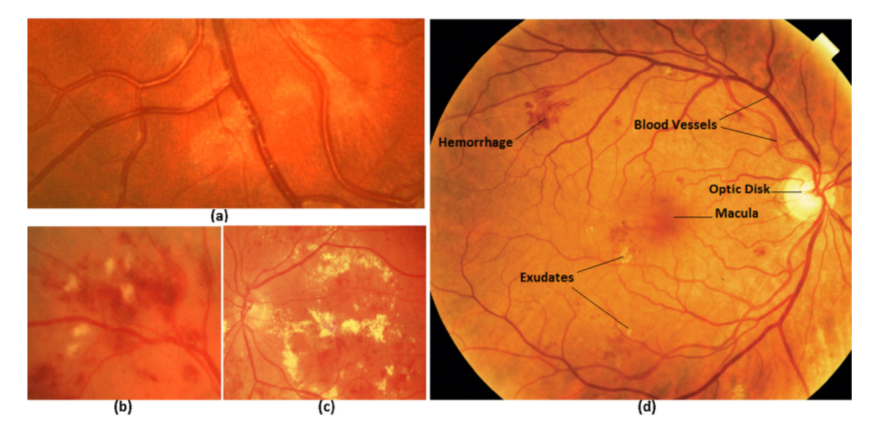
\includegraphics[width=1\textwidth]{Figures/image_ojo}
	\caption[Imagenes de Fondo de ojo]{Morfolog\'ia de im\'agenes de la retina: (a)Reflejo en el vaso central y fondo desigual, (b) Manchas algodonosas, (c)Exudados, (d) Estructura anat\'omica de la retina.}
	\label{fig:Fondo_de_ojo}
	}
\end{figure}	


Los m\'etodos de segmentaci\'on de los vasos de la retina son evaluados en tres bases de datos, DRIVE, HRF y ARIA.

DRIVE es una base de datos a disposici\'on del p\'ublico, que consta de un total de 40 im\'agenes a color con lesiones. Las fotograf\'ias se obtuvieron a partir de un programa de cribado de la retinopat\'ia diab\'etica en los Pa\'ises Bajos.
La poblaci\'on de selecci\'on consisti\'o en 453 sujetos de entre 31 y 86 a\~nos de edad. Cada imagen se ha comprimido JPEG , que es pr\'actica com\'un en los programas de cribado.\\
De las 40 im\'agenes en la base de datos, 7 contienen la patolog\'ia, es decir, los exudados, hemorragias y cambios del epitelio pigmentario. Ver (\ref{fig:Drive_images_retinal}) para un ejemplo de una imagen patol\'ogica y  una normal. Las im\'agenes fueron adquiridas mediante una camara no midri\'atica.\\

\begin{figure}[H]
	{
	\centering
	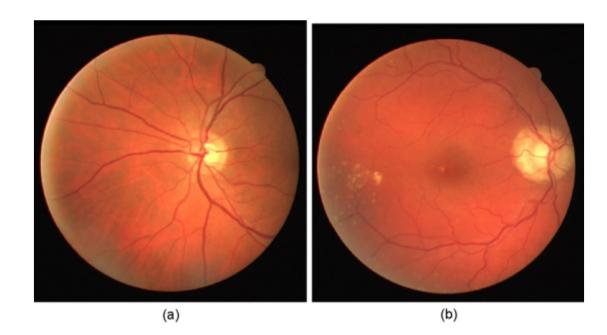
\includegraphics[width=1\textwidth]{Figures/Drive_images_retinal}
	\caption[Drive]{Im\'agen de la retina - DRIVE: (a) Retina saludable, (b) Retina con muestras patol\'ogicas.}
	\label{fig:Drive_images_retinal}
	}
\end{figure}	



En primer lugar, se determinaron los algoritmos a utilizar para mejorar el preprocesamiento de las im\'agenes, es decir, disminuir los efectos secundarios que se generan en la captura de im\'agenes de fondo de ojo como los nombrados anteriormente. 

Para la eliminaci\'on o extracci\'on del ruido se tuvieron en cuenta dos algoritmos: filtro de Difusi\'on Anisotr\'opica y filtro de  Coherencia.\\

En la actualidad existe una  amplia gama de metodologías para la detección automática de defectos  con  bajo contraste, todas ellas dependen de la buena adquisici\'on de la imagen, las condiciones de iluminaci\'on, el tipo de material que se desea inspeccionar, entre otros. A esto se le suma las características de los defectos que se quieran detectar, un ejemplo de estas características es el contraste que generan los defectos con respecto al fondo de la muestra, defectos que generan un mayor contraste son más fáciles de detectar que aquellos cuyo 
contraste es muy bajo.\\
Los defectos de bajo contraste se pueden clasificar dentro de dos clases con características diferentes para las etapas posteriores del proceso como la segmentación y clasificación. En la primera clase se encuentran los defectos oscuros de bajo contraste, estos se caracterizan por tener un nivel de gris más bajo. La segunda clase está conformada por defectos claros con bajo contraste, los cuales tienen un nivel de gris más alto 
en comparación al fondo en el que se encuentran embebidos. Se debe tener en cuenta que los defectos tienen niveles de gris diferentes (mayor o menor) al del resto del objeto de estudio, y  que el bajo contraste del defecto con respecto al  fondo del objeto  hace que la tarea de detección sea compleja tanto para las personas como para los sistemas de inspección industrial basados en visión por computador.\\

Esta secci\'on se centra en la evaluaci\'on del filtro de difusión anisotrópico como estrategia de realzado previa a la segmentación de defectos oscuros de bajo contraste en objetos pequeños de alta reflectividad con iluminación no homogénea.

Definici\'on del modelo de difusi\'on anisotr\'opico\\

La difusión anisotrópica propuesta por Perona y Malik \cite{perona1990scale} está dada de la siguiente manera: 

\begin{displaymath}
I_t=div\lbrack c_t(x,y)\nabla I_t(x,y)\rbrack  \hspace{2cm}(1)
\end{displaymath}

Donde div  es el operador de divergencia, \begin{displaymath}  \Delta \end{displaymath} es el operador Laplaciano y \begin{displaymath}
\nabla \end{displaymath}   es el operador gradiente.  \begin{displaymath} c_t(x,y)\end{displaymath} es el coeficiente 
de difusión definido en función del gradiente de tal forma que se adapte para que los bordes entre regiones sean preservados 
y los detalles intraregiones sean suavizados, \begin{displaymath} c_t(x,y)\end{displaymath} se define como se muestra a continuación:

\begin{displaymath}
c_t(x,y)=g(\nabla I_t(x,y))=1/\lbrack1+(\left|\nabla I_t/k\right|)^2\rbrack \hspace{2cm}(2)
\end{displaymath}

La difusión anisotrópica  se puede expresar de forma discreta de la siguiente manera:

\begin{displaymath}
I_{t+1}(x,y)=I_t(x,y) + \frac14{{{\sum_{i=1}^{4} \lbrack c_t^i(x,y).\nabla I_t^i(x,y)\rbrack}}} \hspace{2cm}(3)
\end{displaymath}

En el modelo discreto \begin{displaymath} \nabla I_t^i(x,y), i= 1,2,3,...,4 \end{displaymath} son los gradientes de los vecindarios en diferentes direcciones y \begin{displaymath} c_t^i(x,y) \end{displaymath} es el coeficiente de difusi\'on mencionado en (2), en esta ecuaci\'on k es una constante que se debe fijar de acuerdo a la aplicaci\'on del filtro seg\'un el desempe\~no que se busque.\\

El filtro de Difusi\'on anisotr\'opica es una técnica destinada a reducir el ruido de una imagen sin necesidad de retirar las piezas importantes del contenido de la imagen, por lo general los bordes, líneas u otros detalles que son importantes para la interpretación de la imagen, el modelo de difusión anisotrópico asemeja el proceso que crea un espacio de escala, donde una imagen genera una familia parametrizada de forma sucesiva cada vez más borrosas de imágenes, basadas en un proceso de difusión.\\ 

EXPLICAR UN POCO MAS DIFUSION ANISOTROPICA

El filtro de Coherencia ...This function COHERENCEFILTER will perform Anisotropic Diffusion of a 2D gray/color image or 3D image volume, Which will reduce the noise in an image while preserving the region edges, and will smooth along
the image edges removing gaps due to noise.\\ HACERLO COMPLETO 



Para la eliminaci\'on o extracci\'on del fondo se tuvieron en cuenta tres filtros denominados de paso bajo, el filtro de mediana, el filtro de media y el filtro gaussiano. 

El proceso de filtrado consiste en la aplicación a cada uno de los pixels de la imagen de una matriz de filtrado de tamaño N x N (generalmente de 3x3 aunque puede ser mayor) compuesta por números enteros y que genera un nuevo valor mediante una función del valor original y los de los pixels circundantes. El resultado final se divide entre un escalar, generalmente la suma de los coeficientes de ponderación. Los filtros se pueden expresar mediante una ecuación (6.1)

\begin{displaymath}
ND'_{i,j}=\frac{ND_{i-1,j-1}+ND_{i,\;j-1}+ND_{i+1,j-1}+ND_{i-1,j}+ND_{i,j}+ND_{i+1,j}+ND_{i-1,j+1}+ND_{i-1,j+1}ND_{i-1,j+1}}9 \hspace{2cm}(6.1)
\end{displaymath}

donde i y j representan la fila y la columna de cada pixel,  \[ND_{i;j}\] su Nivel Digital y \[ND'_{i,j}\] el Nivel Digital obtenido tras hacer el filtrado.\\

El objetivo de estos consiste en suavizar la im\'agen, son útiles cuando se supone que la imagen tiene gran cantidad de ruido y se quiere eliminar. También pueden utilizarse para resaltar la información correspondiente a una determinada escala (tamaño de la matriz de filtrado); 


\begin{itemize}
	\item[$*$] Filtro de la media, asigna al pixel central la media de todos los pixeles incluidos en la ventana. La matriz de filtrado estaría compuesta por unos y el divisor sería el número total de elementos en la matriz.
	
\begin{displaymath}
\begin{array}{l}\begin{array}{cccc}20&23&30&31\\22&21&29&30\\23&24&32&33\\29&31&34&37\end{array}\rightarrow\begin{array}{ccc}1&1&1\\1&1&1\\1&1&1\end{array}\rightarrow\begin{array}{cccc}N&N&N&N\\N&24.8&28.1&N\\N&27.2&30.1&N\\N&N&N&N\end{array}\\\\\;\;\;\;\;\;\;\;\;\;\;\;\;\;\;\;\;\;\;\;\;\;\;\;\;\;\;\;\text{Filtro de Media}\end{array}
\end{displaymath}
				
	\item[$*$] Filtro de la mediana tiene la ventaja de que el valor final del pixel es un valor real presente en la imagen y no un promedio, de este modo se reduce el efecto borroso que tienen las imagenes que han sufrido un filtro de media. Además el filtro de la mediana es menos sensible a valores exremos. El incoveniente es que resulta más complejo de calcular ya que hay que ordenar los diferentes valores que aparecen en los pixeles incluidos en la ventana y determinar cual es el valor central.
\begin{displaymath}
\begin{array}{l}\begin{array}{cccc}20&23&30&31\\22&21&29&30\\23&24&32&33\\29&31&34&37\end{array}\rightarrow\begin{array}{cccc}N&N&N&N\\N&23&30&N\\N&29&31&N\\N&N&N&N\end{array}\\\\\;\;\;\;\;\;\;\;\;\;\;\;\;\;\;\;\;\;\text{Filtro de Mediana}\end{array}
\end{displaymath}

	\item[$*$]Filtros gaussianos. Simulan una distribución gaussiana bivariante. El valor máximo aparece en el pixel central y disminuye hacia los extremos tanto más rápido cuanto menor sea el parámetro de desviación típica s. El resultado será un conjunto de valores entre 0 y 1. Para transformar la matriz a una matriz de números enteros se divide toda la matriz por el menor de los valores obtenidos. La ecuación para calcularla es:
	
	\begin{displaymath}
	g(x,y)=e^{-\frac{x^2+y^2}{2\ast s^2}} \hspace{2cm}(6.2)
	\end{displaymath}
	
	\begin{displaymath}
		G(x,y)=\frac{g(x,y)}{min_{x,y}(g(x,y))} \hspace{2cm}(6.3)
	\end{displaymath}
\end{itemize}


Para mejorar el contraste de las im\'agenes se utiliz\'o la t\'ecnica Contrast Limited AHE (CLAHE), la cual mejora el contraste  de la im\'agen en escala de grises mediante la transformaci\'on de los valores. CLAHE opera sobre peque\'nas regiones de la im\'agen , llamados azulejos , en lugar de toda la im\'agen.El contraste de cada regi\'on es mayor, por lo que el histograma de la zona de salida coincide aproximadamente con el histograma especificado por el parámetro ' Distribución ' . Los azulejos vecinos se combinan a continuación, utilizando la interpolación bilineal para eliminar los límites inducidas artificialmente . El contraste , sobre todo en áreas homogéneas , puede ser limitada para evitar la amplificación de cualquier ruido que pudiera estar presente en la imagen.


Con los métodos de filtrado definidos y analizados teniendo en cuenta sus ventajas y desventajas, se realizaron cuatro pipelines para determinar cu\'al de estos es el mejor para utilizar en los sets de im\'agenes propuestos.

\begin{itemize}
	    \item Pipeline 1 -> Extracci\'on de fondo(Mediana, Media o Gaussiano)  +  Realce(CLAHE)  +  Extracci\'on de ruido(Filtro anisotr\'opico o Filtro de Coherencia)
		\item Pipeline 2 -> Realce(CLAHE) +  Extracci\'on de ruido(Filtro anisotr\'opico o Filtro de Coherencia)
		\item Pipeline 3 -> Realce(CLAHE) +  Extracci\'on de fondo(Mediana, Media o Gaussiano)
		\item Pipeline 4 -> Realce(CLAHE)  + Extracci\'on de fondo(Mediana, Media o Gaussiano)   +  Extracci\'on de ruido(Filtro anisotr\'opico o Filtro de Coherencia)
\end{itemize}






%-----------------------------------
%	SECTION 3
%-----------------------------------

\section{Extracci\'on de caracter\'isticas}


%----------------------------------------------------------------------------------------
%	SECTION 4
%----------------------------------------------------------------------------------------

\section{M\'etodo de segmentaci\'on}

